%!TEX encoding = UTF-8 Unicode
%!TEX root = ../lect-w11.tex

%%%


\Subsection{Generiska strukturer}

\begin{Slide}{Repetition: Typparametrar och generiska strukturer}
\begin{itemize}\SlideFontSmall
\item Med hjälp av \Emph{typparametrar} \Eng{type parameters} kan du skapa \Emph{generiska strukturer} \Eng{generic structures}.
\item Typparametrar skrivs inom hakparenteser, exempelvis: \code{ [T, U] }
\item Generiska strukturer fungerar för \emph{olika} typer, \Alert{okända} vid \Emph{deklaration}. 
\begin{Code}
case class Pair[A, B](a: A, b: B):  // [] gör att A, B är obundna (fria)
  def swap: Pair[B, A] = Pair(b, a) // A och B bundna då swap saknar []
\end{Code}
\pause
\item Kompilatorn säkerställer \Alert{korrekt} \Emph{användning} redan vid \emph{kompilering}.
\item På användningsplatsen i koden (vid anrop eller instansiering) \Emph{binds} typparametrar till ''verkliga'' typer enligt typsystemets regler. 
\begin{REPL}
scala> val p = Pair("hej", 42)
val p: Pair[String, Int] = Pair(hej,42)

scala> p.swap
val res0: Pair[Int, String] = Pair(42,hej)
\end{REPL}
\pause
\item Skriver du inte ut typerna försöker kompilatorn \Emph{härleda} \Eng{infer} dem.
\item Klassen \code{Pair} kallas även \Emph{typkonstruktor} \Eng{type constructor} då den ''verkliga'' typen skapas först vid användning \code{Pair[String, Int]}.
\end{itemize}
\end{Slide}


\Subsection{Att sätta gränser för typer}

\begin{Slide}{Olika sätt att begränsa typer}
Det finns i Scala flera olika sätt att att begränsa vilka typer du vill tillåta. En översikt av några möjligheter:
\begin{itemize}
  \item Ge \Emph{övre} gräns för typparametrar \Eng{lower bound}
  \item Ge \Emph{undre} gräns för typparametrar \Eng{upper bound}
  \item Ge en \Emph{kontextgräns} för typparametrar i relation till implicit givna typer \Eng{context bound}
  \item Begränsa möjlig inmixning vid deklaration av en trait med en explicit \Emph{egentyp} \Eng{self type} 
\end{itemize}
\end{Slide}

\begin{Slide}{Övre och undre typgränser}\SlideFontSmall
Med typoperatorerna \code{<:} och \code{>:} går det att begränsa vilka typer som kan bindas till en typparameter i en generiska struktur. 

\vspace{0.5em}Antag att \code{T} är en obunden typparameter medan \code{U} och \code{L} är bundna. 
\begin{itemize}
  \item med \code{T <: U} blir \code{U} en övre gräns \Eng{upper bound} för \code{T}\\(en ''högsta'' möjliga typ i  typhierarkin) 
  \item med \code{T >: L} blir \code{L} en undre gräns \Eng{lower bound} för \code{T}\\(en ''lägsta'' möjliga i  typhierarkin) 
  \item Minnesregel för typgränser: kolon på slutet.
  \item Alla typer \code{T} är implicit \code{T >: Nothing <: Any}
\end{itemize} 
\pause

\vspace{0.5em}Exempel: 
\begin{Code}
  trait Grönsak { def vikt: Int }

  def f[T <: Grönsak](x: T): Int = x.vikt
\end{Code}

Kompilatorn använder den övre typgränsen för att konstatera att metoden \code{vikt} är tillgänglig via den generiska parametern \code{x}.

\end{Slide}

\begin{Slide}{Exempel på övre och undre typgränser}

\begin{Code}
class Djur
class Katt extends Djur 
class Hund extends Djur
class Robothund extends Hund

def testUpperBound[T <: Hund](x: T) = println(x)
def testLowerBound[T >: Hund](x: T) = println(x)
\end{Code}

\begin{REPL}
scala> testUpperBound[Katt](Katt())
-- Error:
1 |testUpperBound[Katt](Katt())
  |          ^
  |          Type argument Katt does not conform to upper bound Hund

scala> testLowerBound[Robothund](Robothund())
-- Error:
1 |testLowerBound[Robothund](Robothund())
  |          ^
  |          Type argument Robothund does not conform to lower bound Hund
\end{REPL}

\end{Slide}

\begin{Slide}{Typbegränsning med egentyp \Eng{self type}}\SlideFontSmall
\begin{itemize}\SlideFontTiny
  \item Det går att få ett explicit, valfritt namn, t.ex. \code{self},  på ''min egen typ'' genom att skriva~\code{ self => }~i kroppen på en trait eller klass. 
  \item Detta kallas \Emph{egentyp} \Eng{self type}. 
  \item Användbart vid inmixning: du kan begränsa egentypen med en typannotering.
\begin{Code}
trait Grönsak { def vikt: Int }
trait KanSkalas:
  self: Grönsak =>
  def viktEfterSkalning = 0.99 * vikt 
\end{Code}
\begin{REPLsmall}
scala> val g = new Grönsak with KanSkalas { val vikt = 100 }
val g: Grönsak & KanSkalas = anon1@70a91d72
                                                                                    
scala> g.viktEfterSkalning
val res0: Double = 99.0
\end{REPLsmall}
\item Även om \code{KanSkalas} \Alert{inte} gör \code{extends} så är \Emph{ändå} \code{vikt} tillgänglig i dess kropp, eftersom vi kräver att den egna typen är en \code{Grönsak}.
\item Kan användas för att göra s.k. \Emph{beroendeinjektion} \Eng{dependency injection}.\\\url{https://en.wikipedia.org/wiki/Dependency_injection}
\end{itemize}

\end{Slide}



\Subsection{Flexibla generiska typer: varians}

\ifkompendium\else
\begin{SlideSimple}{Vad är varians?}
\hspace*{-2cm}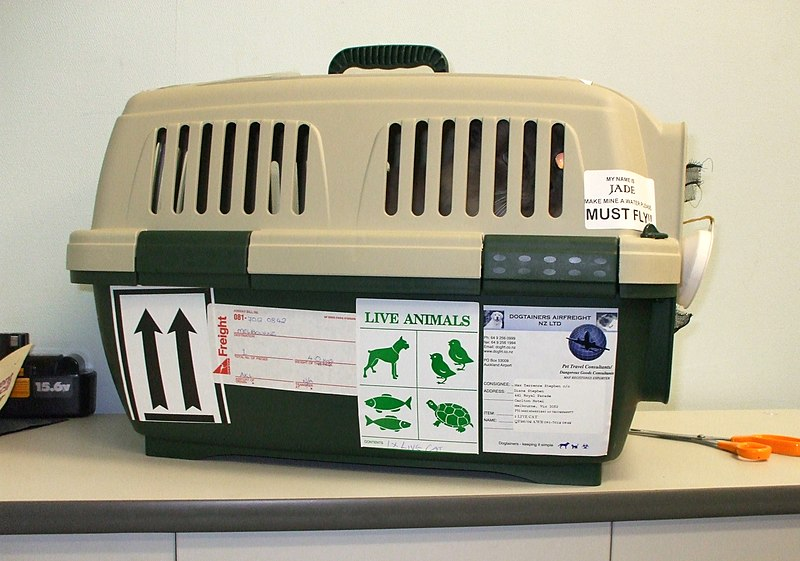
\includegraphics[width=1.4\textwidth]{../img/pet-carrier.jpg}  
\end{SlideSimple}
\fi 

\begin{Slide}{Vad är varians?}
\begin{center}
\textbf{Är en kattbur också en djurbur??}

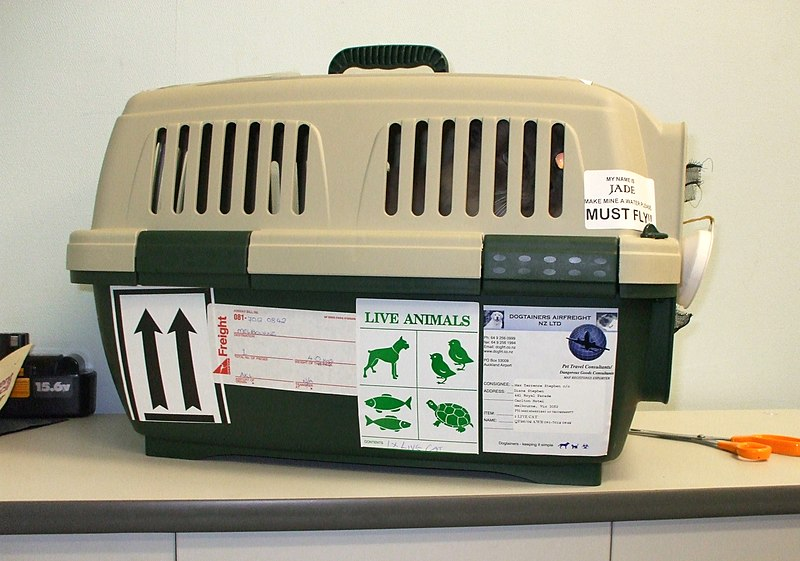
\includegraphics[width=0.75\textwidth]{../img/pet-carrier.jpg}  

Om vi tillåter \Emph{varians} så blir generiska strukturer mer \Alert{flexibla}.
\end{center}
\end{Slide}

\begin{Slide}{Varför behövs varians?}\SlideFontSmall
\begin{Code}
trait Djur
case class Katt() extends Djur
case class Hund() extends Djur

case class Bur[A](a: A)
\end{Code}
\pause
Nedan fungerar inte! Buren ovan är \Emph{invariant} (oflexibel i sin typparameter).
\begin{REPL}
scala> val djurbur: Bur[Djur] = Bur[Katt](Katt())
-- Error:
1 |val djurbur: Bur[Djur] = Bur[Katt](Katt())
  |                   ^^^^^^^^^^^^^^^^^
  |                   Found:    Bur[Katt]
  |                   Required: Bur[Djur]
\end{REPL}
\pause
Varför fungerar detta??
\begin{REPL}
scala> val djur: Vector[Djur] = Vector[Katt](Katt())
val djur: Vector[Djur] = Vector(Katt())
\end{REPL}
\pause \code{Vector} är deklarerad som kovariant och därmed mer flexibel!
\end{Slide}


\begin{Slide}{Kovarians \Eng{covariance}}
\begin{itemize}\SlideFontSmall
\item För en \Emph{kovariant} typkonstruktor \code{F} gäller att: 
\item[] \textbf{om} \code{ T <: U } \textbf{så} \code{ F[T] <: F[U] }~(subtypsflexibel ''på samma håll'')
\item I Scala skapar du en kovariant typkonstruktor med \code{+} före typparametern:
\begin{Code}
trait Djur
case class Katt() extends Djur
case class Hund() extends Djur

case class Bur[+A](a: A)  // kovariant tack vare + före A
\end{Code}
\pause
\item Nu funkar det \code{:)}
\begin{REPL}
scala> val djurbur: Bur[Djur] = Bur[Katt](Katt())
val djurbur: Bur[Djur] = Bur(Katt())
\end{REPL}
\item En kattbur är nu en \Alert{subtyp} till djurbur!
\pause
\item \Emph{Oföränderliga} samlingar görs ofta kovarianta, t.ex Vector, Option.
\item Enumerationer med \code{enum} görs ofta kovarianta:
\item[] \code|enum Bur[+T] { case Bebodd(x: T); case Tom }|
\end{itemize}

\end{Slide}


\ifkompendium\else
\begin{SlideSimple}{Kontravarians}
\hspace*{-1cm}
\includegraphics[width=1.2\textwidth]{../img/cat-vet.jpg}  
\end{SlideSimple}
\fi 

\begin{Slide}{Kontravarians}
\begin{center}
En djurveterinär är en kattveterinär!?


\includegraphics[width=0.75\textwidth]{../img/cat-vet.jpg}  

Ibland vill vi ha variansen på andra hållet.
\end{center}
\end{Slide}

\begin{Slide}{Kontravarians \Eng{contravariance}}
\begin{itemize}\SlideFontSmall
\item För en \Emph{kontravariant} typkonstruktor \code{F} gäller att: 
\item[] \textbf{om} \code{ T <: U } \textbf{så} \code{ F[U] <: F[F] }~(subtypsflexibel ''på fel håll'')
\item I Scala skapar du en kovariant typkonstruktor med \code{-} före typparametern:
\begin{Code}
trait Djur 
case class Katt() extends Djur
case class Hund() extends Djur

class Veterinär[-A]:
  def behandla(x: A) = println(s"frisk: " + x)  // kontravariant med -
\end{Code}
\pause
\item Nu funkar det ''baklänges'' (men inte på andra hållet):
\begin{REPLsmall}
scala> val kattveterinär: Veterinär[Katt] = Veterinär[Djur]()
val kattveterinär: Veterinär[Katt] = Veterinär@77b6d94c

scala> val kattveterinär: Veterinär[Djur] = Veterinär[Katt]()
-- Error:
1 |val kattveterinär: Veterinär[Djur] = Veterinär[Katt]()
  |                                     ^^^^^^^^^^^^^^^^^
  |                                     Found:    Veterinär[Katt]
  |                                     Required: Veterinär[Djur]
\end{REPLsmall}
\end{itemize}

\end{Slide}

\begin{Slide}{Variansproblem}
\begin{itemize}\SlideFontSmall
\item En typparameter kan \Emph{inte} vara kovariant om den sedan används som typ parametertyp för metoder (så kallad \emph{kontravariant position}):
\begin{Code}
trait Djur
case class Katt() extends Djur
case class Hund() extends Djur
\end{Code}
\begin{REPLsmall}
scala> case class Bur[+A](a: A): 
         def bytTill(x: A): Bur[A] = Bur(x)
-- Error:
2 |  def bytTill(x: A): Bur[A] = Bur(x)
  |          ^^^^
  |  covariant type A occurs in contravariant position in type A of parameter x
\end{REPLsmall}
\item Här måste typen tillåtas variera med hjälp av en \Emph{undre gräns}:
\begin{Code}
case class Bur[+A](a: A): 
  def bytTill[B >: A](x: B): Bur[B] = Bur(x)
\end{Code}
\end{itemize}
\end{Slide}

\begin{Slide}{När använda vilken slags varians?}
\begin{itemize}
\item 
\end{itemize}
\end{Slide}


\begin{Slide}{Typjoker \Eng{wildcard type}}\SlideFontSmall
Generiska typer är normalt \Emph{invarianta} och kan därmed inte utan speciella åtgärder variera mellan mer eller mindre specifika typer. %(mer om varians senare).
\begin{REPLsmall}
scala> case class Box[A](a: A)

scala> var xs = Vector.empty[Box[Any]]

scala> def add[A](b: Box[A]): Unit = xs = xs :+ b
-- Error:
1 |def add[A](b: Box[A]): Unit = xs = xs :+ b
  |                                         ^
  |                                         Found:    (b : Box[A])
  |                                         Required: Box[Any]
\end{REPLsmall}  
Till vår räddning: En \Emph{typjoker} \Eng{wildcard type} anges med ett frågetecken och betecknar en helt okänd typ, vars varians ej kontrolleras av kompilatorn.
\begin{REPLsmall}
scala> var xs = Vector.empty[Box[?]]

scala> def add[A](b: Box[A]): Unit = xs = xs :+ b

scala> add(Box(42)); add(Box("hej")); xs
val res2: Vector[Box[?]] = Vector(Box(42), Box(hej))
\end{REPLsmall}
Använd bara typpjoker om det verkligen behövs, eftersom ingen typkontroll alls sker.
\end{Slide}


\begin{Slide}{Mer om varians för den nyfikne}
Fördjupa dig om varians här:\\\url{https://docs.scala-lang.org/scala3/book/types-variance.html}
\end{Slide}



\Subsection{Kontextuella abstraktioner}

 
\begin{Slide}{Kontextuella abstraktioner: \texttt{given}, \texttt{using}}\SlideFontSmall
\begin{itemize}\SlideFontTiny
\item \TODO \code{given} \code{using}
\end{itemize}
\end{Slide}

\begin{Slide}{Kontextgränser}
\TODO \code{T: Ordering}
\end{Slide}





\begin{Slide}{Sortera samlingar: saknad implicit ordning}
\TODO migrera till Scala 3, implicit -> given
\begin{REPL}
scala> case class Gurka(namn: String, vikt: Int)
defined class Gurka

scala> val xs = Vector(Gurka("a", 100), Gurka("b", 50), Gurka("c", 100))

scala> xs.sorted
<console>:15: error: No implicit Ordering defined for Gurka.
       xs.sorted
          ^
\end{REPL}
\pause
Detta kan fixas genom att tillhandahålla en \Emph{implicit} ordning för \code{Gurka}:
\begin{Code}
implicit object minGurkOrdning extends Ordering[Gurka] {
  def compare(x: Gurka, y: Gurka): Int =
    if (x == y) 0
    else if (x.vikt < y.vikt) -1
    else 1
}
\end{Code}
\end{Slide}


\begin{Slide}{Sortera samlingar: given implicit ordning}
\TODO migrera till Scala 3

\begin{REPL}
scala> case class Gurka(namn: String, vikt: Int)
defined class Gurka

scala> val xs = Vector(Gurka("a", 100), Gurka("b", 50), Gurka("c", 100))

scala> implicit object minGurkOrdning extends Ordering[Gurka] {
         def compare(x: Gurka, y: Gurka): Int =
           if (x == y) 0
           else if (x.vikt < y.vikt) -1
           else 1
       }

scala> xs.sorted
res0: scala.collection.immutable.Vector[Gurka] =
        Vector(Gurka(b,50), Gurka(a,100), Gurka(c,100))
\end{REPL}
{\SlideFontTiny Se exempel på olika bekvämare sätt att definiera en ordning för dina egna typer: \\
\url{https://stackoverflow.com/questions/19345030/}}
\end{Slide}


\Subsection{Applikationsprogrammeringsgränssnitt (api)}
\begin{Slide}{Vad är ett bra api?}
\TODO Beskriv kvalitetsegenskaper hos ett bra api\\
\href{https://stackoverflow.com/questions/469161/how-do-you-define-a-good-or-bad-api}{https://stackoverflow.com/questions/469161/how-do-you-define-a-good-or-bad-api}  
\end{Slide}




